\section{Signaltechnik}
Da es in dieser Arbeit darum geht einen Signalsprung zu erzeugen, wird noch einmal die grundlegende Theorie zu Sprungfunktionen und Signalzeiten erl\"{a}utert. Nach der Definition ist ein Signal ein Zeitpunkt zu dem ein wichtiges Ereignis eintritt. In diesem Fall ist das Ereignis ein Partikelsprung. Als Messstelle wird der optische Z\"{a}hler im Messger\"{a}t verwendet, an dem die eigentliche Messung der Partikel stattfindet. Zu Beginn des Systems enth\"{a}lt das Gas, welches den Z\"{a}hler passiert in der Theorie keine Partikel. Der Partikelanteil liegt also bei \(0\) Partikel \(/\) \(1m^3\) Luft. Ist der Partikelstrom komplett aufgebaut und wird in das Messger\"{a}t geleitet, beschreibt der Partikelanteil im Strom einen Sprung auf einen angestrebten Wert.
\\
Bei diesem Vorgang sind allerdings einige Zeiten zu beachten, welche das System und die entstehende Sprungfunktion beeinflussen. Zun\"{a}chst einmal hat das Messger\"{a}t eine Totzeit, welche die Zeit beschreibt, die ein Partikel vom Eingang des Messger\"{a}ts bis zum Zeitpunkt seiner Messung ben\"{o}tigt. Also bis zu dem Zeitpunkt in dem das Auftreten des Partikels in der Sprungfunktion sichtbar wird. Eine weitere Zeitspanne, die ber\"{u}cksichtigt werden muss, ist die Schaltzeit eines Ventils. Nachdem der Strom voll aufgebaut ist, muss der Luftstrom, der in das Messger\"{a}t einstr\"{o}mt umgeschaltet werden auf den aufgebauten Partikelstrom. Dieses Umschalten kostet auch Zeit, je nachdem welcher Schaltmechanismus verwendet wird. Zusammen genommen ergeben die beiden Zeiten die Totzeit des gesamten Systems. Beschrieben wird die Zeitspanne vom Umschalten des Schaltmechanismus bis zum ersten Anstieg der gemessenen Sprungfunktion.
\begin{figure}[H]
        \myfloatalign
        {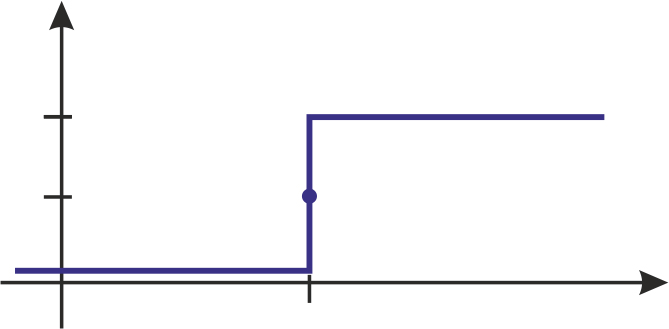
\includegraphics[width=.7\linewidth]{gfx/fundamentals/jump.jpg}} \quad
        \caption[Perfekter Signalsprung]
        {Perfekter Signalsprung}
        \label{fig:sprung}
\end{figure}